\chapter{Conclusion and Final Thoughts}
\label{ch:conclusion}

\vspace{-1cm}
\begin{center}
Eduard Hirsch
\end{center}

This last chapter discusses the goals reached as well as the problems encountered during the development of the INTERLACE prototype. Additionally, it emphasises possible enhancements necessary and issues which need to be taken into account in order to bring the prototype to production level. Finally, it discusses parts that could not be finished as well as after-INTERLACE goals.

\section{Best Practices, Falsey and Pitfalls}

When using Hyperledger Composer but also when connecting to Hyperledger Fabric directly, it is important to take care of some points. Developers have to be aware that working with chaincode or smart contracts is quite different from accessing data as usual in a RDBMS,\footnote{Relational Database Management System} even though up-to-date frameworks  shield a lot of the complexity underneath. Thus, even though access to the data structures and virtual machine/execution capabilities looks similar from a developer's point of view, it is necessary to account for some peculiarities related to blockchain-based technologies, because of their highly distributed nature. In the following sections we discuss and attempt to clarify some of these peculiarities.

\subsection{Deterministic Execution}

One of the most important things to keep in mind when writing chaincode applications is the deterministic execution of transactions. Although it seems quite obvious at first, it can be quite challenging to achieve.

One example is the \textbf{generation of IDs}:  in a standard database environment simple locking mechanisms are in place to ensure correct primary keys for entries in a table. For blockchains which live in a distributed, consensus-based system it is problematic to create identifiers over chaincode execution. The reason is that each peer processing a transaction would compute a new ID completely independently, and most likely at the about the same time. Thus, if such a key-/ID-generation created different IDs on different clients, it might not be possible to reach consensus; thus, although nothing is actually wrong with the transaction itself, the resulting blockchain states in each peer would be different and therefore the last action would be rolled back.

This would be especially hard to deal with during race conditions, and even more difficult to find out why a particular problem has occurred.

One solution to this problem could be to generate the ID from the client and pass it to the transaction as parameter. This would result in a much safer creation process which, additionally, is much faster during execution.

Another problem is posed by the use of \textbf{random numbers}. Since such calculations would reach different results on the various peers of the network, it is impossible to use random numbers in chaincode executions. Further, since it is not possible to know when a peer in the network will receive a new transaction, also the \textbf{creation of a date} or a timestamp is intrinsically random. Thus, dates created by different peer nodes during chaincode execution are different and when written into an e.g.\ asset also create different blockchains on different nodes, and would therefore be rolled back.

For example, a possible scenario is that the date has been chosen to contain only day, month and year, such that execution of many transactions is likely to happen on the same day. In such a case, even if peers were able to reach consensus, validation of the blockchain nodes retroactively would not be possible \textcolor{green}{as the date has been changed completely} and re-executed code results in a different outcome.

\textcolor{red}{I have reworked your new text, please check that what I wrote is still correct. However, I do not understand why the date has been changed completely... . I think you are saying that random date generation would give different results, which would make sense, but it is not clear to me why the date would be randomly chosen. I think some information is still missing from this explanation.}

To sum up the above statements: \textbf{Chaincode needs to be executed deterministically and has to reach, given its input parameters, the same result(s) on all the peer nodes at any point in time}.

\textbf{Note:} Another consequence of this statement is that many parameters cannot be generated by chaincode but need to be provided as parameters to a transaction. But since this means that the parameters are creatable on the client-side only, it is also necessary to implement the corresponding logic in a way that prevents them from being used to fool the system or bring it into an inconsistent state.

\subsection{Network Upgrade}

Traditionally, updating a database after changes to the database model may be quite cumbersome due to the presence of new fields, foreign keys, and many other similar issues. However, various methods and strategies are in place for handling these issues.
On the other hand, since blockchains are usually spread over various peers that store replicated data, in contrast to traditional databases it is inherently more difficult to change the distributed structures to fit some new schema necessary to add a new feature or functionality.

Updating or changing values of asset attributes, as well as getting executable code and data structures ready for the next version of the network, may run into several problems. In particular, in order to maintain consistency and reliably achieve all fixes it is necessary to apply all changes to the network in such a way that upgrading the business network (CTO-File, chaincode, ...) and fixing the asset values happen in the right order, \st{were} \textcolor{red}{and while} nobody else is able to interfere. \textcolor{red}{This can be achieved by executing the upgrade as a single atomic transaction or, if that's not possible, by blocking common user access during deployment.}

\st{Thus, this may happen during a single atomic transaction or, if possible, by e.g. blocking common user access during deployment.}

Thus, it is quite important to get everything right from the beginning, as it can be extremely difficult to apply certain changes. Consequently, it is highly advisable to think about possible changes and future scenarios together with possible side-effects and costs before first deployment to production systems.

\subsection{Hyperledger Composer Specifics}

Composer can be seen as a rapid-development approach. Its API sits on top of the Hyperledger Fabric framework. It tries to shield complexity from the user and aims to significantly reduce the time necessary to create distributed applications for Hyperledger Fabric.

For the development of the INTERLACE transactional service this meant that:
\begin{quote}
\begin{itemize}
	\item models could be transferred easily,
	\item chaincode could be based on these models,
	\item a REST Server was supplied and
	\item a web-application generator was available.
\end{itemize}
\end{quote}

Consequently, it was an ideal framework for prototyping. In addition, once a suitable cloud provider has been found, spinning up a network is straightforward. When hosting a network without an external provider who knows how to run these networks, much of the initial speed in creating it might be lost because, in such a case, a much deeper understanding of the whole architecture is necessary. Thus, also a greater effort is needed to get a ready implementation to work.

\textbf{Note:} For production systems it would be necessary to change to a plain Fabric implementation because Composer is still at quite an early stage of development, and there are even rumours that it may be discontinued. The reason is that some of the new features of the Fabric releases are deviating from the structures implemented by Composer. So it is becoming increasingly difficult for Hyperledger Composer developers to provide new features and functionalities available for Fabric.

\section{Identity Management}
\label{sec:id-management}

As mentioned in previous sections, we skipped Identity Management for the prototype in order to simplify the environment, decrease development efforts and therefore offer a relatively easier access to an example mutual credit system, hoping that this would make it easier to understand the basics. Nevertheless, it would be possible and quick to create additional participants and grant them access to the network in addition to just the currently used admin account. For example, an identity card can be issued for the first participant defined in transaction "InitBlockchain" which is identified by "m1". The example below illustrates how this might be done:

\begin{lstlisting}[language=bash]
	composer identity issue -c admin@tutorial-network -f m1.card -u m1 -a "resource:net.sardex.interlace.Individual#m1" -x true 
\end{lstlisting}

This identity card is facilitated by the REST server and corresponds to a participant in the business network. 
But, when accessing the REST server, before a user can act with that identity it is necessary for him/her to log in first and authenticate his/her identity in some sort of way. To do so composer-rest-server uses an authentication middleware implemented in JavaScript called \textit{Passport.js}.\footnote{\url{http://www.passportjs.org/}}

The passport middleware offers many different authentication strategies and is quite a mature Open Source framework. An example of how to authenticate with OAuth and GitHub can be found on the Composer documentation website;\footnote{\url{https://hyperledger.github.io/composer/latest/integrating/enabling-rest-authentication}} but also different schemes can be used, like the JSON Web Tokens (JWT\footnote{\url{https://jwt.io/}}) which is mentioned in the issue tracker of the Hyperledger Composer GitHub page.\footnote{\url{https://github.com/hyperledger/composer/issues/2038}}

Passport is a commonly known middleware for authentication and may be applied also to different scenarios. Thus, it is usable well also if Composer is swapped for another technology.

\section{Future Scenarios}
\label{sec:future-scene}

Because we are using Hyperledger Fabric, extending the network is only a matter of changing the configuration. The approach taken for the INTERLACE prototype, shown in Figure \ref{fig:prototype-net-ext}, creates a new organisation for every payment circuit that deals with a new specific region. Consequently, each region would be responsible for hosting their own peers and ideally also their own certification authority (CA). However, certificates might be still handled by the Sardex CA. 

Sardex, in this scenario, is providing the network architecture and transferring the know-how about how to run a circuit, which would result in a model similar to a franchise. Although the clients and various other visible graphical interfaces may be branded in various ways, the underlying platform infrastructure would be predefined by Sardex in order to make the network work consistently.

The orderer will be handled by Sardex as well, but later might be handed over to an e.g.\ non-profit organisation representing the circuit and enforcing fair and clearly defined rules within a governance framework defined in collaboration with the circuit members themselves. To ensure a reliable system and a high performance throughput, an orderer could be clustered locally but also over various regionally separated areas.

\begin{figure}[htbp]
  \centering
  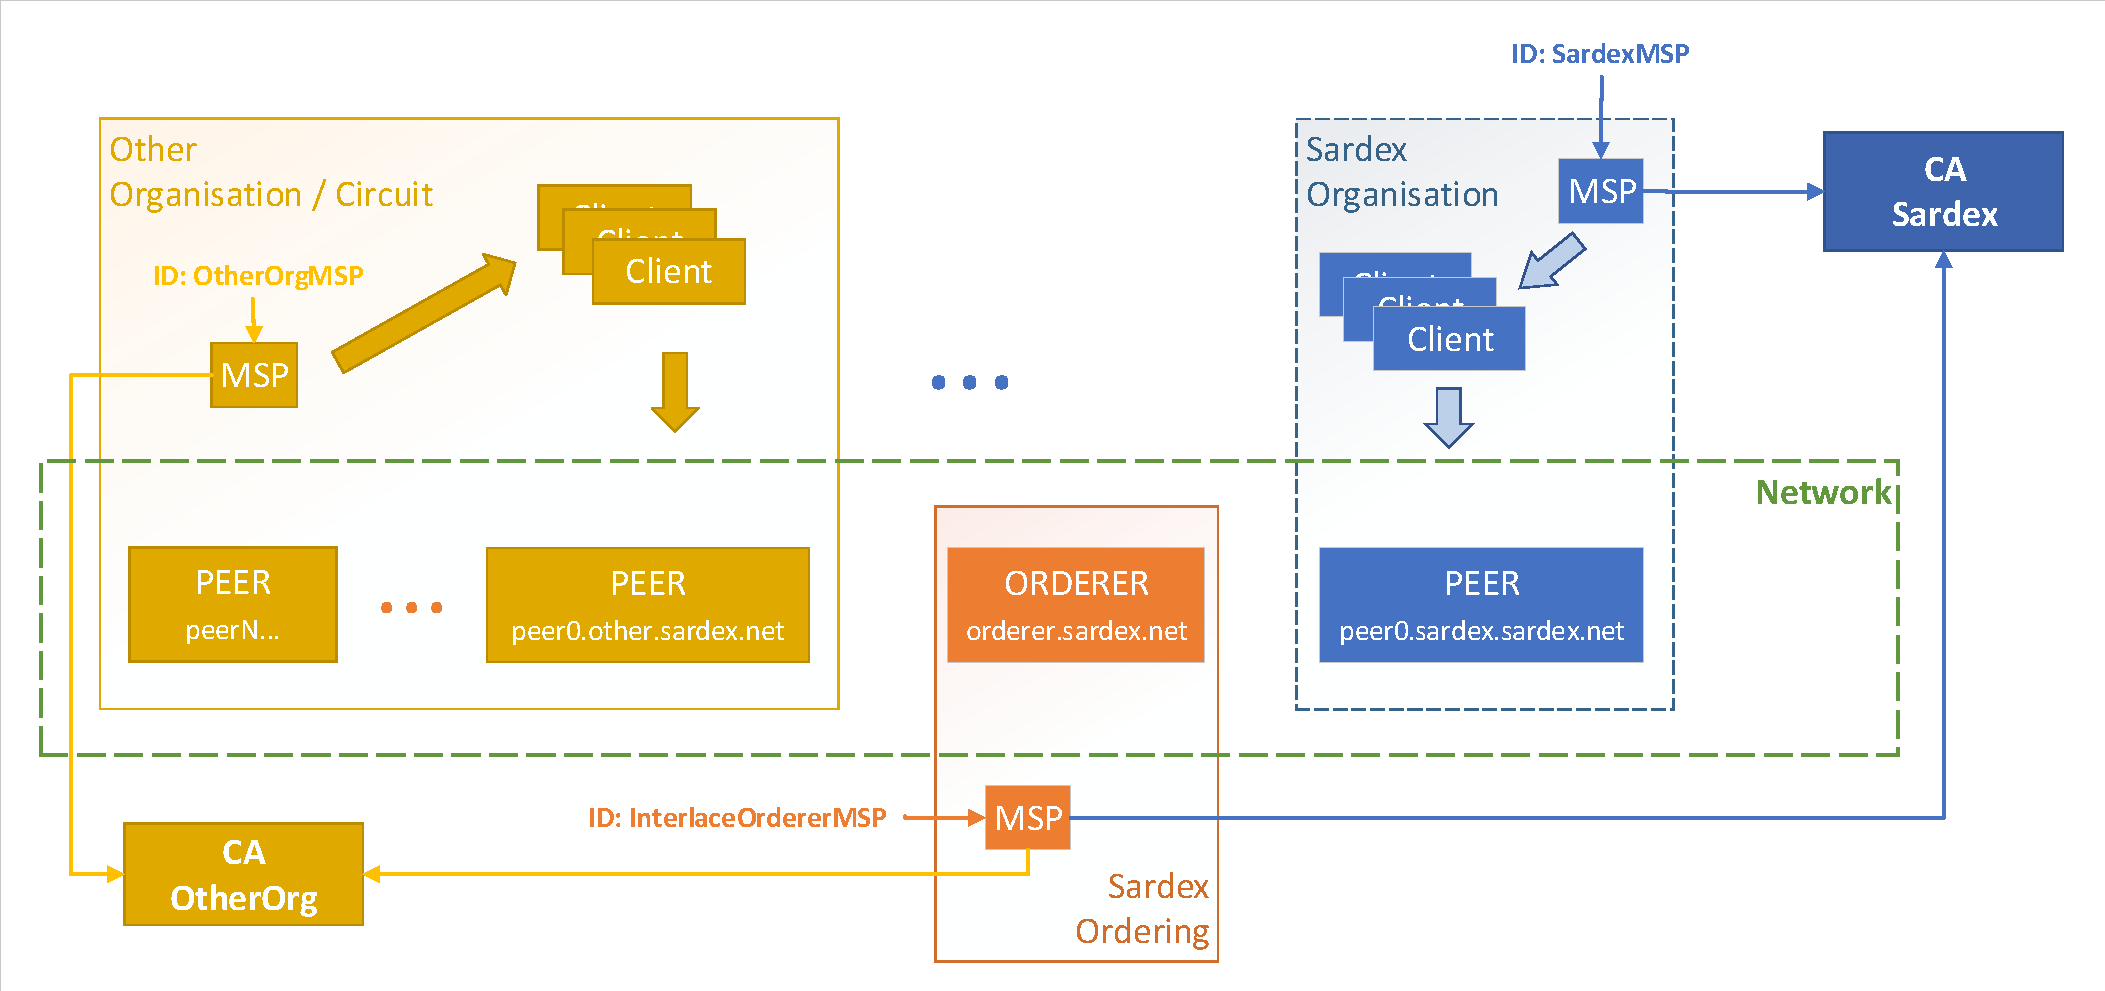
\includegraphics[width=1.0\textwidth, clip, trim=1mm 1mm 1mm 1mm]{Figures/extended-network}
  \caption{\bf\small Extended Network Structure}
  \label{fig:prototype-net-ext}
\end{figure}

\section{Final Review and Open Points}

Our DLT application prototype forms a stable and scalable basis for a reliable payment circuit. In fact, although the prototype was developed with Hyperledger Composer, which IBM may discontinue support for, any subsequent implementation in Hyperledger Fabric only will now be much easier to realize. This is also because newer versions of Fabric support a node.js SDK,\footnote{Software Development Kit} which would even allow the transfer of JavaScript code bits.

In summary, the goal of creating a reliable DLT has been achieved, and forms a necessary foundation for the various other services provided in future for the production-level business solutions created by and with Sardex.

\subsection{Open Points}

The \textbf{GDPR}\footnote{General Data Protection Regulation \cite{GDPR}} directive that came into effect in the first half of 2018 represents a challenge for blockchain solutions and, therefore, also for the INTERLACE project. It is necessary that personal information is not exposed to other parties unless necessary and unless it is done in agreement with its owners. In addition, each piece of information collected for the user or provided by the user needs to be deletable if the user requests it, and it must certainly be possible to look up upon request exactly what data was collected.

Information is reliably stored inside of a blockchain. Thus, looking up information is actually not an issue. Rather, one of the challenges is to keep it secret from being read by other parties, since standard blockchain approaches copy everything to every peer. Another challenge is the immutability of most blockchains, since GDPR enforces the right to be forgotten. The privacy aspect is solved currently by making the actual chain only accessible by the peers that are owned by the organisation running the local circuit. In this configuration, the clients that perform transfers have restricted access and cannot see the whole blockchain.

In later stages it may be possible for every business/party participating in the payment network to access the blockchain directly, i.e.\ to run a node. In this case the so-called \textit{SideDB}\footnote{\url{https://hyperledger-fabric.readthedocs.io/en/latest/private-data/private-data.html}} can be taken into consideration because it is a way offered by Hyperledger Fabric to store information which is only known by the respective client and only shared if permitted by the client.

\textit{SideDB} also solves the problem of GDPR-relevant data because, first, it is only exposed ``to whom it may concern'' and, second, it can be purged without making the chain invalid. The reason is that in SideDB only hashes of transactions and data are stored on the chain, which still makes it verifiable by regenerating the hash and comparing every time a datum needs to be verified. Normally the data only needs to be provided if specifically asked for, e.g.\ in case of an (external) audit.

The second point which needs further effort is the part of the testing coverage where the \textbf{ASIM implementations} are \textbf{tested} against the actual implementation of the prototype and later against the production-level implementation. These tests will be covered in deliverables D4.1 and D4.2 whose future versions will be completed after the end of the project.






